
In this chapter the ``detectors' gaps problem'' in Bragg Coherent Diffraction Imaging and our approach to solve it
using Deep Learning are discussed. The main state-of-the-art measures are presented briefly and
the topic of image inpainting with Deep Learning is introduced. The focus will then shift to our works that led
eventually to the optimal ``Patching-based'' approach that can also be found in the published paper entitled
 \textit{``Patching-based deep learning model for the Inpainting of Bragg Coherent Diffraction patterns affected 
 by detectors' gaps''} (\url{https://doi.org/10.1107/S1600576724004163}). The chapter is closed with some analyses 
 of the performances of the DL models in a variety of simulated and experimental cases.  

\section{The ``Gap Problem''}\label{sec:gaps}

At time of writing, standard BCDI experiments employ pixelated photon counting detectors to acquire the diffraction
patterns. These detectors can guarantee high spatial resolution, noise-free counting and fast read-out times. Two examples 
of these devices, currently used at the ID01 beamline are the MAXIPIX and EIGER detectors \cite{ponchut_maxipix_2011, Eiger_Johnson_2014}.
These detectors are often built by tiling together several sensing chips in order to cover a larger area, and are
typically bonded to an Application-Specific Integrated Circuit (ASIC) using bump bonding. 
This implies the presence, in the overall sensing region, of vertical and/or horizontal stripes that are not sensitive
to the impinging radiation. The width of these lines varies depending on the device but normally does not exceed the equivalent 
of some tens of pixels. Specifically, for the MAXIPIX detector the gap size is of 6 pixels while the EIGER has larger gaps of both
12 pixels and 38 pixels.
The detector gaps problem does not affect BCDI only, but it is shared among other x-ray techniques that deal with single photon-counting
pixelated detectors and/or beamstops.
We have seen in chapter \ref{chp:intro} that during a BCDI scan the 2D images acquired by the detector are stacked to form
a 3D array. This leads these lines to become planes of missing signal in the dataset.
The problems arise when reconstructing the data affected by these gaps. In fact, these regions of non-physical zero intensity
deceive the Phase Retrieval algorithms inducing the presence of artifacts in the reconstructions\cite{carnis_towards_2019}


\begin{figure}
    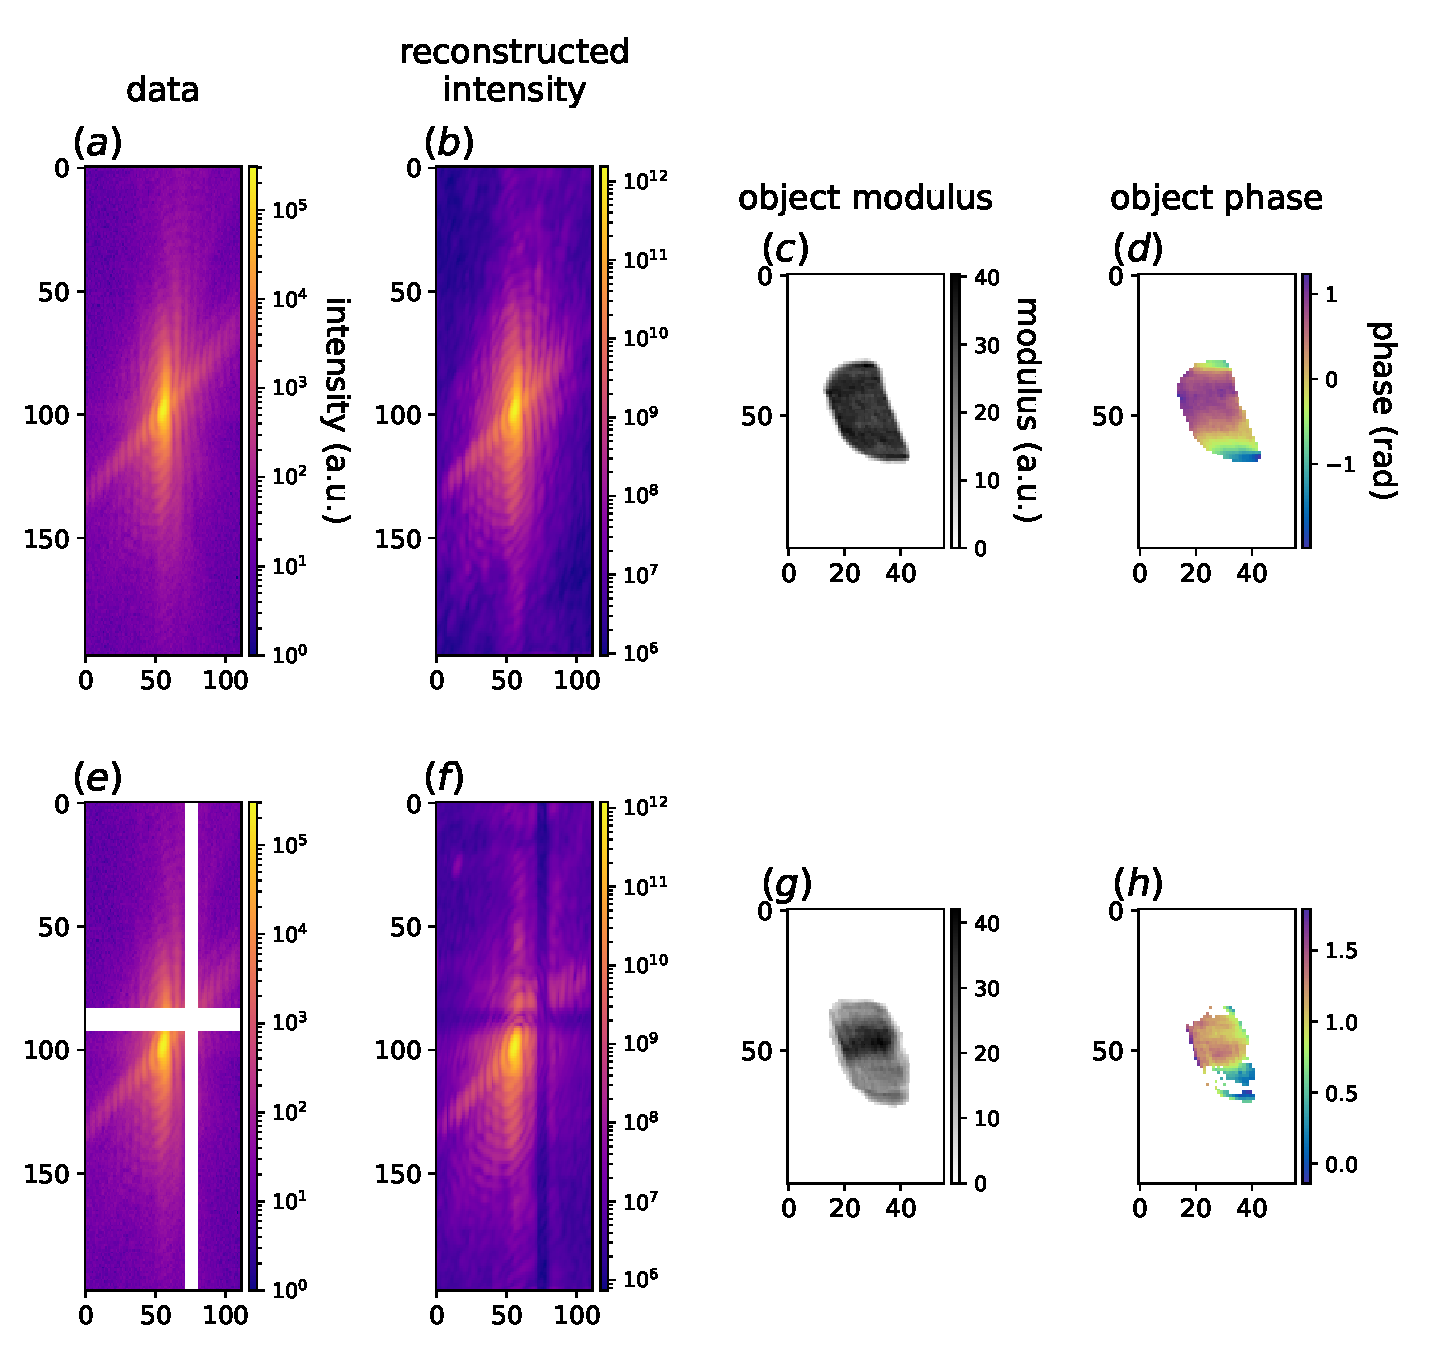
\includegraphics[width=\textwidth]{figures/Inpainting/gaps_intropdf.pdf}
    \caption{\textbf{Effect of detector gaps in BCDI reconstructions} 
    \textbf{(a)} The central xz slice of an experimental diffraction pattern. \textbf{(b)} The same slice of the diffracted
    intensity calculated from the retrieved object. \textbf{(c - d)} xz slice of the modulus and phase respectively of the particle
    obtained from the phasing of the gap-less dataset. \textbf{(e)} Same slice as in \textbf{(a)} with an artificially added
    6 pixel-wide, cross-shaped gaps to mimic the detector's ones. \textbf{(f)} The same slice of the diffracted
    intensity calculated from the retrieved object when not masking the gap regions. \textbf{(h - g)} xz slice of the modulus and phase respectively of the particle
    obtained from the phasing of the gap-affected dataset. The distortions caused by the gaps are evident. }
    \label{fig:gap_intro}
    \end{figure}


It follows that the reliability of the reconstructions in this case is 
compromised as the strain distribution can be deeply affected by the artifacts. A good practice during standard BCDI experiments
is to avoid the gaps by moving the detector if possible. However, this tends to be problematic for the case of high-resolution BCDI, 
i.e. when the diffraction pattern measurement extends to higher q-values, thus covering more than one sensing 
chip and necessarily crossing a gap region. Under these circumstances it becomes important to reduce the amount of
artifacts deriving from the gaps. 


\section{State of the art}\label{sec:InpStateArt}

Here we will discuss the current strategies employed to treat the detector gaps. As someone could argue, the simplest
yet not practical, solution would be to slightly move the detector sideways and acquire a second full scan with the
gap hiding a different region of the same Bragg peak, and then merge the two measurements into a single gap-less one. 
This would in turn increase the acquisition time of more than 2X making it de facto never an option during standard experiments. 
Iterative phasing algorithms like PyNX allow the user to define a mask of the gap regions and will.


\section{Model design}\label{sec:model}
\section{Patching approach}\label{sec:patching}
\section{Results in detector space}\label{sec:res_rec}
\section{Results in real space}\label{sec:res_real}
\section{Fine-tuning}\label{sec:finetuning}
\section{Performances assessment}\label{sec:performances}
